\subsection{Mediator Pattern}


\subsubsection*{Problembeschreibung}

Große Softwareprojekte bestehen meist aus einer großen Anzahl von Klassen bzw. Objekten, welche miteinander interagieren. Ziel ist es stets, die Kopplung zwischen diesen Komponenten so lose wie möglich zu halten, um die Übersichtlichkeit des Codes zu bewahren. Komplexe Interaktionsmuster zwischen diesen Objekten lassen sich nicht immer verhindern, da sie die inhärente Komplexität des modellierten Problems wiederspiegeln. In diesem Fall ist eine Lösung notwending, die diese Komplexität kapselt. Das \emph{Mediator Pattern} ist in der Lage, solche Fälle von komplexer Interaktion zu vereinfachen. \cite{gamma_design_1995}

\subsubsection*{Lösung}

Der konkrete \emph{Mediator} (\code{ConcreteMediator}) implementiert die \emph{Mediator}-Schnittstelle (\code{Mediator}), welche die Methode \code{notify} bereitstellt, um Benachrichtigungen der einzelnen Komponenten (\code{Component}) entgegenzunehmen. Jede Komponente besitzt eine Referenz auf den \emph{Mediator}, um \code{notify} an ihn senden zu können. Dabei übergibt die Komponente sich selbst, um dem \emph{Mediator} den Kontext der Benachrichtigung bereitzustellen. In Abhängigkeit von dem übergebenen Sender und dessen Zustand, führt der \emph{Mediator} eine (komplexe) Logik aus, welche vollständig innerhalb des \emph{Mediators} gekapselt ist. Der \emph{Mediator} hält ebenso Referenzen auf alle Komponenten, die er zu beeinflussen in der Lage sein soll. Die gekapselte Logik kann somit die Interfaces der Komponenten verwenden, um diese zu beeinflussen. Dadurch findet eine indirekte Beeinflussung von Komponenten durch andere Komponenten über den \emph{Mediator} statt. Das Klassendiagramm dieser Architektur ist in \autoref{fig:mediator-class} dargestellt.

\begin{figure}[!ht]
	\centering
	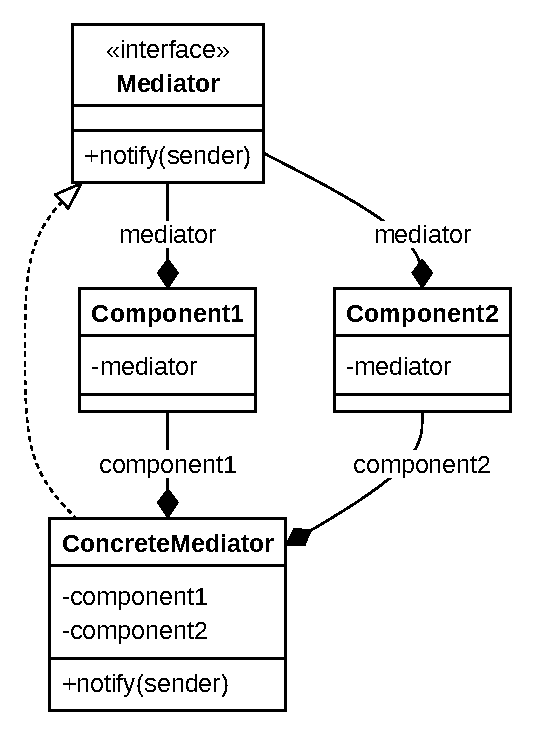
\includegraphics[width=0.75\linewidth]{images/patterns/mediator-class.pdf}
	\caption{Klassendiagramm des \emph{Mediator} Patterns. Die Komponenten kommunizieren nur über den konkreten \code{Mediator} miteinander. Er dirigiert die Interaktion zwischen den Komponenten. \cite{skobeleva_mediator_2023}}
	\label{fig:mediator-class}
\end{figure}

\subsubsection*{Konsequenzen}

Der \emph{Mediator} kapselt Verhalten, welches ansonsten über mehrere Klassen verteilt wäre. Soll dieses Verhalten spezialisiert werden, so ist nur eine Spezialisierung des \emph{Mediators} notwendig. Weiterhin verhindert der \emph{Mediator} eine starke Kopplung der Komponenten. Komponenten- und \emph{Mediator}-Klassen können bei kompatiblen Interfaces beliebig ausgetauscht werden. Der \emph{Mediator} vereinfacht außerdem die Multiplizitäten von Objektinteraktionen. Er wandelt $m$:$n$- Beziehungen zwischen Objekten in $1$:$n$-Beziehungen zwischen den Objekten und dem \emph{Mediator} um.

Der \emph{Mediator} bündelt Kontrolle an einem einzigen Punkt. Dies kann zur Übersichtlichkeit beitragen, kann dieser jedoch bei ausreichend komplexer Logik auch entgegenwirken. Das kann dem \emph{Mediator} eine monolithische Struktur geben, deren Verhinderung seine eigentliche Aufgabe ist.

Sind die Abhängigkeiten zwischen den Komponenten zu Komplex, so kann das \emph{Observer Pattern} zur Kommunikation zwischen den Komponenten und dem \emph{Mediator} verwendet werden. Dadurch lassen sich die Abhängigkeiten außerdem flexibler gestalten, sie können also zur Laufzeit einfacher geändert werden. \cite{gamma_design_1995}